\chapter{Digital Education Technologies and Sustainability}
\label{cha:2_dets-and-sustainability}
The purpose of this chapter is to present the definition of Digital Education Technologies (DETs) and the impact that digitalization has on higher education institutions. 

Section \ref{sec:2.1_DETs} derives the definition of Digital Education Technologies and Sustainable Digital Education Technologies from the literature. Section \ref{sec:2.2_digitalization} discusses the phenomenon of digitalization, focusing on the role of cloud infrastructures in the academic context and the related consequences. Finally, Section \ref{sec:2.3_sustainability_dimensions_DETs} identifies the sustainability dimensions for digital education technologies.

% Idea
% Digital Edcation Technologies
% Sustainable DETs
% Digitalization: context and problems
%   Privacy concerns and missing power on institutions
%   Vendor lock-in
% Sustainability dimensions (Purvis) 
% % The problem of DETs selection: tehnical and pedagogical dimensions

\section{Digital Education Technologies}
\label{sec:2.1_DETs}
Over the past few decades, digital education technologies (DETs) have been subject to continuous development and widespread adoption by higher education institutions, driven by their potential to expand learning and teaching opportunities and meet many global goals in education \cite{volery_critical_2000}.
The term ‘digital education technologies’, often also called 'edtech’, refers to hardware and software resources that produce, share, and store information electronically, supporting and improving learning efficiency, academic productivity, outcomes, and accessibility \cite{sokhulu_students_2021}. 
The use of these technologies in higher education began in the early 1990s alongside the rapid development of Information Technology (IT). They were originally intended as computer-based teaching, with a clear focus on pedagogical practices. Then this concept has grown, spreading into the daily lives of students and teachers, facilitating content sharing, communication, administrative tasks, and even the enrollment of students \cite{lacka_examining_2021}. The first evolution of DETs is represented by learning management systems (LMS) such as Moodle and Blackboard, which enabled structured course management, resource distribution, and student interaction within digital learning environments. The growing popularity of the Internet and mobile devices led to the development of new technologies, including video-conferencing tools, Massive Open Online Courses (MOOCs), and virtual classrooms\cite{haleem_understanding_2022}. As a result, digital education technologies (DETs) are now an essential component of students’ learning experiences. \\
Since its introduction, edtech has become a focus of research, revealing its beneficial and detrimental effects\cite{lacka_examining_2021}. DETs have been claimed to improve teaching and learning processes, potentially leading to better student learning outcomes. In addition, approaches that involve digital technologies (e.g., blended learning) have been argued to broaden accessibility, enhance inclusion, and improve academic performance \cite{tulinayo_digital_2018}. On the other hand, it has been argued that the use of digital education technologies may have harmful effects on students, as many of them lead to inconsistent results \cite{lacka_examining_2021}.
One of the most important criticisms of these tools is that there is still a lack of focus on pedagogical practices and on students themselves.

\subsection{Sustainability in Higher Education}
In recent decades, sustainability awareness has become increasingly important. The way we use this term today is highly influenced by the 1987 UN Commission on Environment and Development, which provided a definition of sustainable development that later became a principle for many scholars, organizations, and governments \cite{correia_sustainability_2019}. 
As a result, the concept of sustainable education emerged, attracting significant interest from researchers. Around 20 years ago, Velázquez et al. proposed a systematic procedural framework for higher education institutions to improve their environmental, social, and economic performance. Their work introduced a clear definition of a sustainable university, describing it as an institution that seeks to minimize negative environmental, economic, and social impacts while fulfilling its core functions of teaching, research, outreach, and stewardship \cite{velazquez_sustainable_2006}. 
Since the concept of sustainable universities emerged, research in this field has been widely centered on integrating sustainability principles into higher education systems, such as reducing the carbon footprint of campuses, improving energy efficiency, incorporating sustainability into academic programs, and fostering education for sustainable development. The introduction of the Sustainable Development Goals (SDGs) in 2015 by all member states of the United Nations (UN), particularly the Quality Education target, broadened the scope of research, emphasizing the need for a more accessible and inclusive education and the potential of digital learning tools to facilitate the achievement of these goals.

\subsection{Sustainable Digital Education Technologies}
The SDGs aim to "ensure inclusive and equitable quality education and promote lifelong learning opportunities for all" \cite{united_nations_goal_2015}. This objective has significantly influenced the concept of sustainable education, steering the focus toward a more socially aware approach. While remarking on the need to reduce the environmental impact and promote sustainable development, it highlights the importance of an education system that is safe, accessible, effective, and free of disparities. Although the study of DETs and sustainable education is widely diffused, a well-known definition of sustainable DETs is still missing.
%Clearly, digital education technologies play a crucial role in advancing the Quality Education target of Sustainable Development Goals.
In this study, the term "Sustainable Digital Education Technologies" is used to encompass the established definition of digital education technologies, while also integrating the broader concept of sustainability across all stages of their lifecycle. For example, using videoconferencing tools to host lectures can reduce the environmental impact of students reaching campus while simultaneously improving accessibility to scholars who cannot attend in person \cite{grebennikova_sustainable_2021}.
% REQUIRE ATTENTION: work in progress section


\section{Digitalization of European Universities}
\label{sec:2.2_digitalization}
Nowadays, digital technologies have become the norm in higher education. The underlying reason for the spread of education technologies lies in the phenomenon of the digitalization of universities. The digitalization of higher education institutions refers to the increasing adoption and integration of digital and computer-based technologies into university operations, teaching, learning, research, and administration \cite{schuetze_digitalization_2024}. While universities have historically been pioneers in deploying and maintaining their own digital infrastructure, most of them are now joining the trend of outsourcing their self-hosted assets to cloud-based infrastructures - including server hardware, email services, shared storage, and video conferencing. \cite{angeli_conceptualising_2022}. This process of outsourcing has evolved gradually over the years, often without a systematic needs assessment or long-term strategic planning, and was further accelerated by the COVID-19 pandemic \cite{schuetze_digitalization_2024}.

%\subsection{The pandemic-effect and the shift to Big Tech}
\subsection{The shift to Big Tech cloud providers}
A recent trend in higher education is the shift of essential digital services, such as email, learning management system, and administration tools, as well as learning-oriented digital tools, toward cloud infrastructures. This migration finds its roots in the large-scale proliferation of Software as a Service (SaaS) and the promise of public cloud providers to deliver cost-efficient and highly scalable cloud solutions. \cite{fiebig_heads_2023}.

The COVID-19 pandemic and the resulting global lockdown forced universities to rapidly adopt external services to ensure the swift resumption of academic activities through flexible teaching methodologies. As a consequence, the pandemic served as a catalyst for accelerating the ongoing outsourcing process of  digital infrastructures and services to cloud providers. This rapid shift led to the centralization of both digital infrastructure and service provision, which has primarily benefited private for-profit technology corporations (Big Tech) \cite{angeli_conceptualising_2022}. The privatization of university digital services offers clear short-term benefits, such as reduced operational costs for service maintenance and the management of qualified staff. However, it also introduces several challenges, ranging from the loss of institutional autonomy to diminished control over data governance.

The profit-driven nature of Big Tech companies prioritizes monetization and their business interests over the educational mission of higher education institutions, seeking to increase the dependency of universities and strengthen their influence over them. Service providers and universities are legally bound by contracts and terms of service agreements that specify data ownership, service conditions, and subscription costs. A common practice among platform owners is to impose long-term contractual obligations, making it difficult for universities to exit agreements or transition to alternative services. Even when exiting is legally possible, technical lock-in mechanisms come into play, making migration harder due to economic and operational constraints \cite{komljenovic_rise_2021}. The cloud platform market for host university infrastructure is almost monopolized by a few actors, such as Google, Amazon, and Microsoft, who often offer digital solutions with limited adaptability and extensive use of proprietary standards. \cite{fiebig_heads_2023}. Moreover, the outsourcing process has reduced universities' internal capabilities, both in terms of digital infrastructure and qualified IT staff, making a return to an on-premise scenario highly unlikely.

The widespread adoption of DETs has also intensified concerns about privacy, data security, and data ownership. Since their introduction, companies have actively promoted edtech solutions as tools to enhance learning outcomes and boost student engagement. Although education technologies undeniably play a key role in the achievement of many educational goals, corporations often overstate them as a one-size-fits-all solution, simplifying the concept of learning to align with their technological and economic interests rather than the pedagogical needs of teachers and students \cite{teras_post-covid-19_2020}. With increasing digitalization, universities are losing control over user data, as ownership is transferred to external entities that freely collect, process, and store it according to their own values and policies. This loss of control raises concerns about the misuse of the collected data, which becomes a valuable asset to enhance market competitiveness rather than to serve educational and pedagogical goals. In fact, data collection is not limited to learning analytics, but potentially extends to personal information and metadata as well. Even though universities have their own data protection policies, they often end up aligning with the provider’s terms of service, making user acceptance a necessity rather than a meaningful choice. For example, Zoom was almost the standard videoconferencing tool for distance learning delivery during the pandemic, and students had no real choice: they had to use the platform, along with the consequent collection of their personal data, or be excluded from lectures \cite{fiebig_heads_2023}.

Ethical concerns about cloud-based solutions have also highlighted important considerations regarding the environmental impact of digital infrastructure. Big Tech companies have been know to make false claims about their greenhouse gas emissions \cite{obrien_data_2024}, and their lack of transparency complicates efforts to estimate the environmental footprint of the digital infrastructure. Furthermore, the continuous increase in software system requirements accelerates hardware obsolescence, shortening its lifespan and contributing to the generation of electronic waste \cite{angeli_conceptualising_2022}. As a result, universities face growing challenges in independently assessing the environmental impact and shaping effective sustainability policies.

%The global lockdown and the urgent need to deliver education through flexible teaching methodology forced educational institutions to rapidly shift to online learning. As a quick solution, European universities accelerated their outsourcing process toward Big Tech companies cloud providers, such as Zoom, Google and Microsoft. These centralization of services and infrastructure, has primarily benefited private, for-profit technology corporations \cite{angeli_conceptualising_2022}.

\subsection{The need for a critical shift in DETs procurement}
As broadly discussed in the previous section, the current approach to the selection of DETs in higher education is strongly driven by economic considerations, as it tends to prioritize vendor convenience and short-term cost savings over institutional autonomy. The increasing reliance on external cloud providers appears to be related to long-term strategic IT decisions rather than being a reactive response to the pandemic, which instead has contributed to the acceleration of the process \cite{fiebig_heads_2023}.

\begin{figure}[ht!]
  \centering
  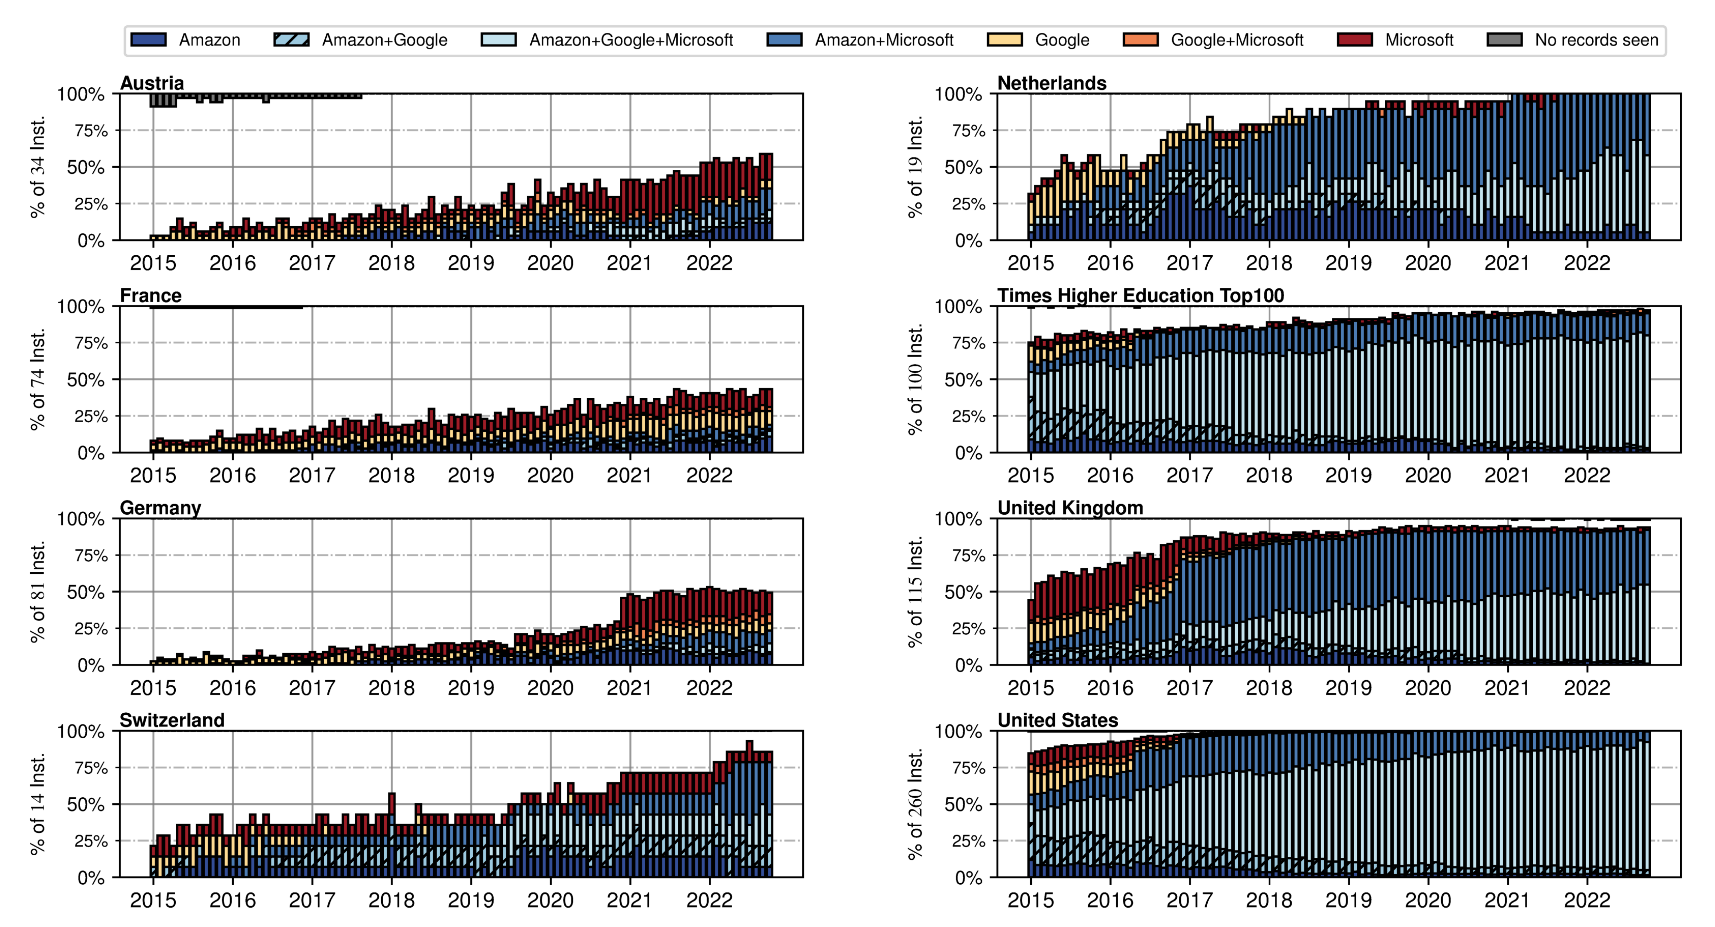
\includegraphics[width=0.9\textwidth]{img/digitalization_erupean_hei_fiebig.png}
  \caption{\centering{Increasing use of external cloud providers by European universities from January 2015 to October 2022 \cite{fiebig_heads_2023}.}}
  \label{fig:digitalization_european_universities}
\end{figure}

Some existing and ongoing studies agree on the potential risks and long-term implications that digitalization imposes on educational institutions. They suggest that self-hosting practices could be a viable solution for universities to regain control over their digital infrastructure. The use of Free/Libre Open Source Software (FLOSS), at least for critical digital services, can enhance transparency and provide guarantees regarding the proper use of data. FLOSS adoption and self-hosting represent an opportunity for universities to play an active role in developing and maintaining solutions that align with their institutional needs. Moreover, contributing to and adopting FLOSS solutions can help build strong internal capacity and foster greater technological independence and autonomy. Clearly, self-hosting requires significant long-term investments, and the optimized cost-efficiency implied by cloud resource dynamic allocation and the pay-as-you-go model is not comparable in the short term. However, as internal personnel expertise grows, the outcome may prove a more sustainable option, potentially reducing costs over time \cite{fiebig_heads_2023}. Additionally, research encourages universities to prioritize solutions that promote pedagogical values and view open-source solutions and self-provision as an ethical alternative to the current trend.

In support of the research, Huang M., in his extensive study involved some northwestern European universities, confirmed that economic considerations still represent a major factor in DETs procurement, often justified by limited financial resources and a lack of human resources. Although environmental sustainability is considered an important requirement, the lack of environmental impact metrics and the challenges in obtaining data tend to overshadow it, leading institutions to prioritize other sustainability aspects \cite{huang_building_2023-1}.

It is evident that there is a need for a critical shift in edtech procurement. Further research could make a major contribution to addressing and analyzing the new challenges and the ethical concerns created by digital education technologies \cite{teras_post-covid-19_2020}. 

\section{Sustainability dimensions for DETs}
\label{sec:2.3_sustainability_dimensions_DETs}
Among the hundreds of definitions associated with sustainability, the concept of sustainable development, introduced by the Brundtland Report \cite{are_1987_nodate}, remains the most widely recognized and accepted. It is defined as "meeting the needs of the present without compromising the ability of future generations to meet their own needs". However, its context-specific nature prevents it from being reduced to a single, universal definition. Sustainability is often depicted as an interdependent relationship between three distinct dimensions: economic, social, and environmental \cite{purvis_three_2019}. The foundational concept underlying the three-pillar model is the necessity of balancing the three aforementioned dimensions, in contrast to the assumption that economic growth alone can ensure sustainability and long-term prosperity. Treating these dimensions as isolated concerns can have detrimental effects. Disregarding the environmental dimension can result in increased pollution, excessive resource consumption, and climate change while exacerbating social inequalities. On the other hand, ignoring the social dimension may affect social well-being, contributing to weakened economic productivity and subsequent environmental degradation due to unsustainable practices.

A closely related popular framework that applies sustainability principles in a business-oriented context is Elkington's Triple Bottom Line (TBL), which extends the traditional bottom line of financial performance by incorporating social and environmental factors (People, Planet, Profit - 3P) \cite{correia_sustainability_2019}. The model encourages organizations to integrate corporate social responsibility initiatives into their decision-making processes, such as ensuring people's welfare as well as their contribution to the community. The model also incentivizes minimizing the environmental footprint, addressing the problems of energy consumption, waste production, and the use of natural resources. However, the framework is primarily designed to evaluate business performance in terms of measurable output and has been criticized for favoring the economic dimension over the social and environmental ones. This often leads companies to superficially address sustainability while maintaining a primary focus on profit.

\begin{figure}[ht!]
  \centering
  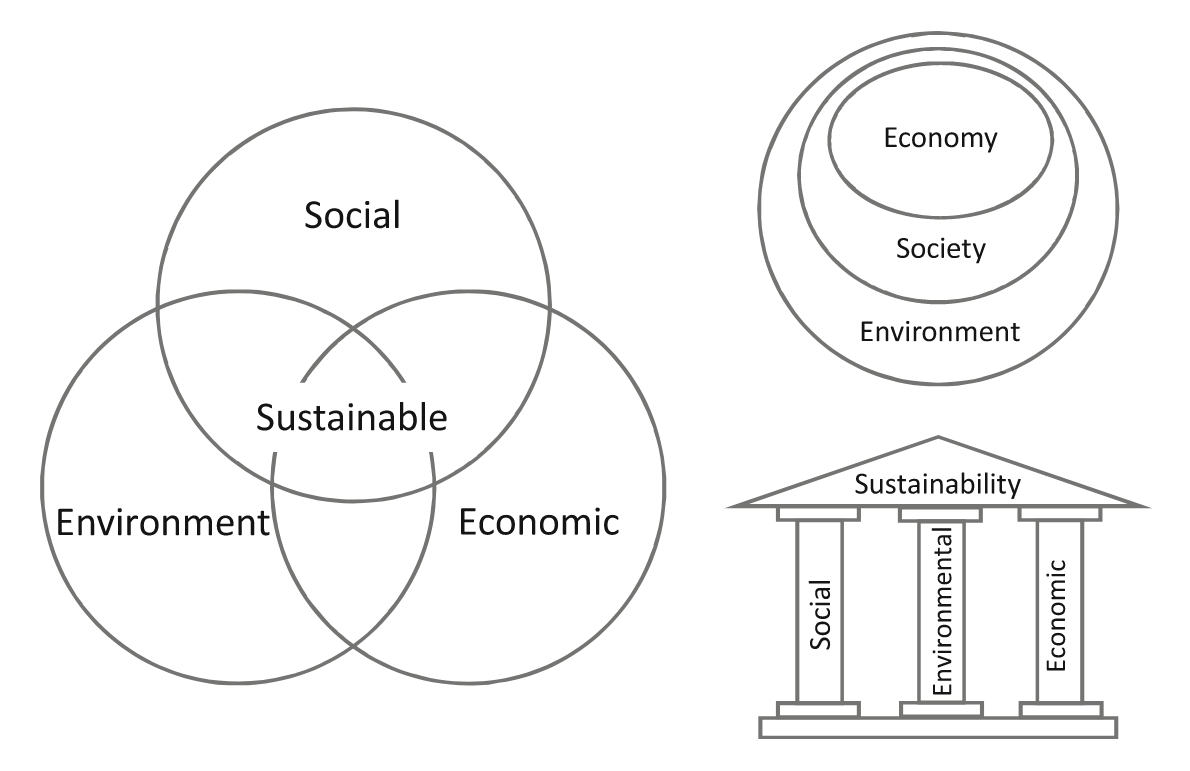
\includegraphics[width=0.6\textwidth]{img/three_pillars_model.png}
  \caption{\centering{Common representations of sustainability: (from left) overlapping circles, structural pillars, and a hierarchical model \cite{purvis_three_2019}.}}
  \label{fig:three_pillars_model}
\end{figure}

It is evident that the TBL model is not well suited for assessing the sustainability of digital education technologies. The selection process for education technologies requires a broader evaluation of social and ethical aspects that go beyond the business-oriented focus of this framework. Moreover, key factors such as pedagogical effectiveness and accessibility do not align with the dimensions proposed by the triple bottom line. Additionally, its emphasis on profitability contrasts with the financial dynamics of universities, which are geared toward economic feasibility and resource management.

The holistic approach suggested by the three-pillar concept represents a more appropriate solution for the selection process of digital education technologies. By extending the traditional framework to include pedagogical and technical dimensions, it provides a more comprehensive evaluation method that aligns with the specific needs of higher education institutions. This expanded model will serve as the foundation for the framework developed in this thesis, ensuring a sustainability-driven approach that aims to balance all the dimensions at stake.